\chapter{Implementation}\label{sec:implementation}
\section{First approach}
The original source code of QCADesigner was downloaded from Mina website (\cite{site:QCADesigner}). We attempted to make it compile as it was but we did not
manage to solve several compilation errors. So we started to focus on the identification of the core algorithm supporting the tool in
order to obtain a working batch simulator executable on CPU. This operation took us some weeks of work. Meanwhile we were able to deeply
analyze the code. We made some hypothesis on the location of possible bottlenecks, we identified the data structures used to represent 
circuits and started to consider possible transformations that had to be done in order to obtain fast accessible and light weight data 
structures allocable on the GPU global memory.

\section{The CPU algorithm and code analysis}\label{sec:cpu_algorithm}
Bistable engine is thought as a fast and approximated simulation, sufficient to verify the logic functionality of a design. 
Every cell is represented as a simple two-state system. The entire simulation is divided into samples, that are units of time 
(not yet experimentally defined), and for each sample the state of each cell is calculated with respect to the other cells within 
a preset effective radius. This operation is iterated until all cells have converged within a predetermined tolerance. 
Once the entire system converges the output is recorded and the computation goes on with the next sample, after having updated
 the input cells with new input values.
The number of samples required to have a good approximation is known (\cite{site:MinaBistable}) to be $2000*2^N$, where $N$ is the number of inputs.
 The maximum number of iterations allowed for the convergence within a sample is set to $100$. Thus, during a simulation each cell's value 
is computed sequentially $It*2000*2^N$ times, where $It$ is the mean number of iterations needed to reach convergence. 
The more are the cells, the longer will take each sample to reach convergence. Each cell's new state calculation implies several accesses to the memory, since data structures are heavily dereferenced, and each neighbor's state as well as their reciprocal kink energy has to be read, and a series of floating point operations on values with double precision. Furthermore, at the beginning of each sample, new inputs values have to be set. As far as exhaustive simulation is concerned, every combination of input values has to be processed. Therefore, their values are calculated through a periodic function, implying several transcendental functional unit usages.\newline
The analysis of the code makes it quite clear that the core of the simulation is the main bottleneck of this application. Once a circuit of millions of cells have to be simulated, the number of FP operations and memory accesses reach huge orders of magnitude. This first hypothesis was subsequently proved by the profiling of execution times, dealt with in section \ref{sec:cpu_profiling}.

\begin{algorithm}[h!tb]
  \dontprintsemicolon
  \SetKwData{NumSamples}{numberOfSamples}\SetKwData{MaxIter}{maxIterations}\SetKwData{NumColors}{numberOfColors}\SetKwData{Stable}{stable}
  \SetKwData{NCellLayers}{nCellLayers}\SetKwData{NCellsPerLayer}{nCellsPerLayer}
  \SetKwFunction{MemcpyToGPU}{MemcpyToGPU}\SetKwFunction{MemcpyToCPU}{MemcpyToCPU}\SetKwFunction{UpdateInputs}{UpdateInputs}
  \SetKwFunction{ComputePol}{ComputePolarization}\SetKwFunction{Randomize}{RandomizeCells}
  \SetKwFunction{GetPolarization}{Polarization}\SetKwFunction{CollectOutputs}{CollectOutputs}
  \SetKwInOut{Input}{input}\SetKwInOut{Output}{output}\SetKw{KwAnd}{and}\SetKw{KwNot}{not} 
  \SetKwFor{While}{while}{do}{endw}
  \KwData{$NewP:$}
  \BlankLine
  \For{$j\leftarrow 0$ \KwTo \NumSamples}
  {
    \UpdateInputs{$Pol$}\;
    \Randomize{$Pol$}\;\label{alg:rand}
    $i \leftarrow 0$\;
    $stable \leftarrow false$\;
    \While{$i<$\MaxIter  \KwAnd \KwNot $stable$}
    {
     \For{$k \leftarrow 0$ \KwTo \NCellLayers}
      {
	\For{$l \leftarrow 0$ \KwTo \NCellsPerLayer}
	{
	  $OldP \leftarrow$ $Pol_{k,l}$\;
	  $NewP \leftarrow$ \ComputePol{$Pol_{k,l}$}\;
	  $stable \leftarrow$ (($|NewP - OldP| < tolerance$) \KwAnd $stable$)\;\label{alg:tolerance}
	  $Pol_{k,l} \leftarrow NewP$\;
	}
      }
     }
   \CollectOutputs{$Pol$}\;
  }
  \caption{Original Bistable Engine Pseudocode}\label{algo_bist_serial}
\end{algorithm}


\section{Profiling of CPU simulation}\label{sec:cpu_profiling}
Once the batch application was finished we started to profile the execution times simulating some circuits of different sizes and different number of inputs. The table \ref{tab:cpu_profiling} shows the results we obtained. We calculated the mean number of iterations per sample needed to reach convergence, the core simulation time, the time of the entire simulation, including data loading from file and creation of data structures, and the proportion of the computation that we aim to speedup.
\newline
\begin{table}[h!tb]
   \centering \caption{CPU simulation Profiling}
   \label{tab:cpu_profiling}
   \vskip 0.2cm
   %%
   \scalebox{0.90}{
	    %% The {|c|c|c|c|c|} define the number of columns.
	    %% c means centered
	    %% | defines a vertical line between two columns 
	    \begin{tabular}{|c|c|c|c|c|c|}
	      \hline
	      Cells & Samples & Iter. per sample & Core Time & Total Time & P \\
	      \hline
	      35576 & 8000 & 10.16 & 2590 s & 3106 s & 83.3 \% \\
	      \hline
	      35486 & 16000 & 12 & 5642 s & 6165 s & 91.5 \% \\
	      \hline
	      31875 & 32000 & 11 & 8668 s & 9078 s & 95,4 \% \\
	      \hline
	      35893 & 64000 & 11 & 20799 s & 21335 s & 97.5 \% \\
	      \hline
	      24498 & 128000 & 11,5 & 25324 s & 25544 s & 99.1 \% \\
	      \hline
	    \end{tabular}
	 }
 \end{table}
As we can see, the hypothesis we made about the bottleneck is verified. Furthermore, the proportion of the computation for big circuits get bigger with the number of samples used, so with the number of inputs. The maximum expected improvement is, according to Amdahl's Law: $ \frac{1}{(1-P)+\frac{P}{S}} $, where S is the maximum speedup achievable parallelizing the portion P. For big circuits we can consider $P=1$ and thus the speedup of the entire simulation is equal to the speedup we manage to obtain from the parallelization of the core simulation.

\section{Parallelization Strategy}
\subsection{The new algorithm and achievable speedup}\label{sec:new_algorithm}
As we have seen in section \ref{sec:cpu_algorithm}, the calculation of the each cell's new state is immediately stored before proceeding with the next cell. Therefore, not all of the new polarizations computation is based on the old value of neighbors. This dependence challenges our seek of the maximum speedup, since our initial proposal was to compute every cell's new state simultaneously. The figure \ref{fig:cpu_alg} shows how this dependency affects a simulation step varying the order in which the cells are considered.
\begin{figure}[h!tb]
	\centering
	\subfigure[First order]{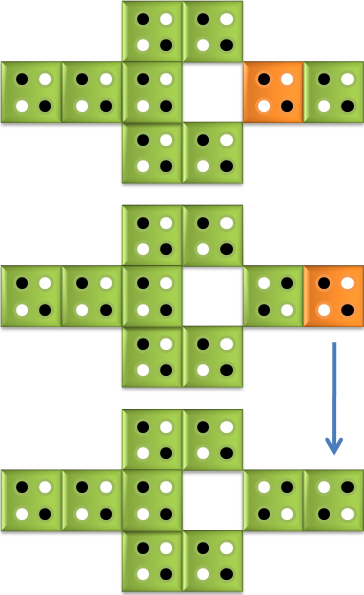
\includegraphics[scale=0.4]{img/CPUalg1.png}}
	\subfigure[Second order]{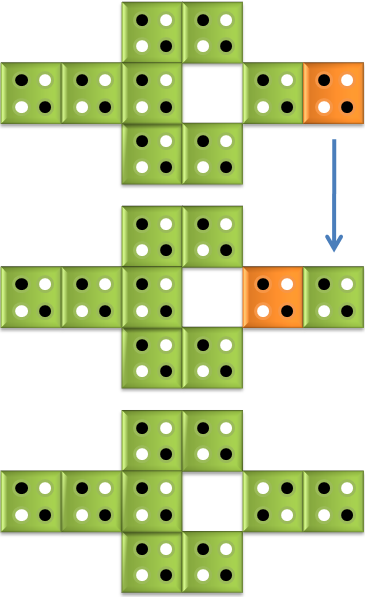
\includegraphics[scale=0.4]{img/CPUalg2.png}}
	\caption{New state computation with different orders}
	\label{fig:cpu_alg}
\end{figure}
We initially made the hypothesis that calculate the new state of a cell entirely based on the old state of the neighbor cells would have worked even better than the current algorithm. This way we would have had a maximum speedup achievable of the core simulation proportional to the number of the cells.
Given our lack of competence in this field, we contacted Professor Konrad Walus of the University of British Columbia (Canada), which is the head of the Microsystems and Nanotechnology Research Group (MiNa) which developed this tool. He sustained our hypothesis, adding that their implementation was different just because copying each value would have worsen considerably performances on CPU, and that any numerical problem that may incur is bypassed by randomizing each sample the order in which cells are considered.\newline
As far as coherence engine is concerned, this was true, and the team which is working on it had brilliant results with this algorithm. Unfortunately, the bistable simulation gave us an unexpected result: the state of the system did not converge to a stable state, on the contrary, cells' state starts oscillating and oscillations seems to get larger after some iterations. This result is probably due to the fact that this kind of simulation is just an approximation of the dynamic of the system and what happens is something comparable to the latch SR when is goes from the \textit{forbidden state} $R=S=1$ to the \textit{keep state} $R=S=0$, whose output is unpredictable and the result will depend on the propagation time relations between the NOR gates. In our case, the algorithm is trying to compute the new state not considering any analogue relaxation time difference. Obviously this problem occur only when making logical approximations. The coherence engine is a physical simulation, so this problem is overcome.

\subsection{Parallelization by labels}
In order to find a working parallelizable algorithm, two approaches had been considered then. The former was to modify someway the computation of the new state, in order to overcome any sort of oscillation and maintain the before prospected speedup roof, the second was to consider the dependency that was discussed in section \ref{sec:new_algorithm}, affecting negatively the achievable speedup.
As for the first option, we tried adding some noise or skipping randomly the new polarization update when an oscillation is individuated, but we did not succeed. Again because of our lack of competence, we showed this problem to the MiNa group and we are currently in contact with a PhD which actively contributed to the creation of this tool. Meanwhile we managed to obtain a working bistable simulator exploiting the second option.\newline
In order to maintain the dependency of the original algorithm we decided to divide the entire circuit into labels so that every cell has no neighbors on his label and computing simultaneously not all the cells, but cells belonging to the same label.
The neighborhood relationship is stored as an undirected graph. Applying a coloring algorithm on it, we obtained these labels. Our graph has some peculiarity which had to be considered in order to find a fast and efficient coloring algorithm:
\begin{itemize}
	\item The graph is undirected, but as for \textit{fixed} and \textit{input} cells (whose values do not depend on the other cells state) it is directed, since we decided to mark these kind of cells as if they have no neighbors, while a normal cell is allowed to have them as neighbors;
	\item A \textit{fixed} and \textit{input} cell is allowed to have any color;
	\item A normal cell is allowed to have the same color of his neighbor if this neighbor is a \textit{fixed} and \textit{input} cell;
	\item The maximum number of arcs does not scale with the number of cells since there is a predefined effective radius within which the number of cells that can be located is physically bounded.
\end{itemize}
Therefore, we preferred to implement a home made coloring algorithm, which has a linear complexity and gives a small number of colors in a really short time. The graph \ref{fig:color_table} shows the trend of the number of colors found in some circuits in relation to the number of cells.
\begin{figure}[h!tb]
				\centering
				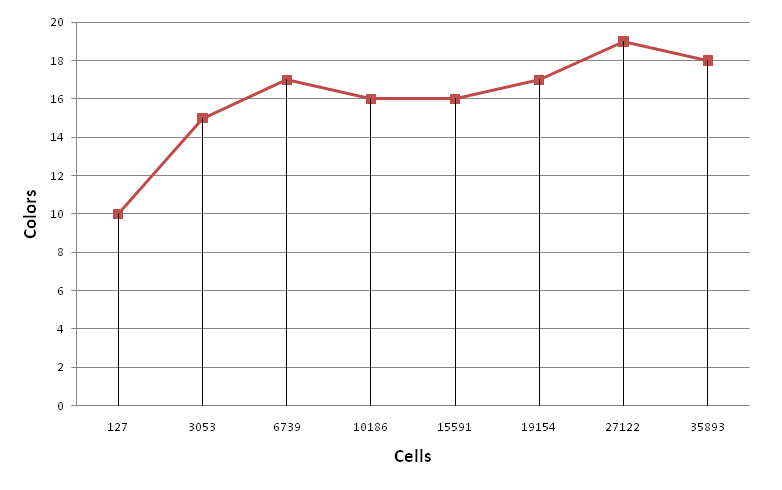
\includegraphics[scale=0.5]{img/color_table.png}
				\caption{Number of colors found with our coloring algorithm.}
				\label{fig:color_table}
\end{figure}
Obviously it also depends on the structure of the entire circuit, but here is shown how the last property we pointed out makes the maximum number of colors well bounded by a limit of about 20-25 colors.\newline In order to avoid numerical errors, the randomization of the cells' order would be too time expensive because of the many memory transfers that would be required between host and device. With this new algorithm, things become easier since it is sufficient to randomize the color order every sample so that the there is no predefined sequence of labels being computed.\newline
This way a sequentiality is introduced and the maximum speedup achievable is inevitably worsen, but still our maximum speedup will be proportional to the number of cells as the circuit get bigger, since we can consider as a constant the number of colors.

\subsection{Data Structures}
In the CPU implementation all the information about circuit structure and cells' details are stored in complex nested and dereferenced structures:
considering CUDA SIMT parallelism, well suited to operate over structures like matrices and arrays, we first detected the useful data
for simulation on GPU and then decided how to organize them for a fast CUDA implementation.\newline
The essential data we identified were: cells' polarizations, neighbors' lists, intra-cells kinetic energy (\textit{eK}) values, clock values,
stability status and other predefined constants.\newline
We decided to store most of these values (the ones that ) in simple array structures, in order to obtain a clearer thread mapping and a faster thread access.\newline
Cells' polarizations array is in charge of containing the polarization values for all the cells through all the iterations, providing
the results for simulation output. At each iteration, polarizations are updated by threads.\newline
Neighbors' and \textit{eK} arrays contain all the informations we need about circuit structure and energy interactions among
the cells. They fully depend on circuit's geometry, and do not change during the simulation. However, they are essential to calculate 
cells polarizations.\newline
Stability array contains simple boolean values which provide the stability status of every cell and permits the evaluation of array global
stability after every iteration.\newline
Other significant structures we designed in our implementations are the input and output cells' indexes arrays, two auxiliary structures
which help us respectively to update input cells at the beginning of every sample and to store output cells' polarization at the end of 
every iteration.

\subsection{Parallel Algorithm}
As reported previously, in our parallel implementation we focused our attention on the simulation core of the algorithm.\newline
Our goal was to exploit the parallel thread execution to compute simultaneously all the circuit's cells. 
After the initial circuit file reading and structures filling phases, we introduced a conversion function to have data in our desired format.
After conversion the coloring algorithm is applied and all the needed data are ready to be allocated on the device.\newline
Parallel bistable simulation, could be divided into the below stages:
\begin{itemize}
 \item allocation and copy of the variables on the device, which is performed only one time during the execution.
 \item update inputs kernel, executed at the beginning of each sample to update inputs.
 \item bistable kernel, invoked in every iteration as many times as the number of colors in the circuit
 \item stability checking, performed after each iteration
 \item copy-back of output cells polarizations from device to host, necessary to save circuit output at the end of each sample
 \item cleaning device memory after the last sample.
\end{itemize}

\begin{algorithm}
  \SetKwData{NumSamples}{numberOfSamples}\SetKwData{MaxIter}{maxIterations}\SetKwData{NumColors}{numberOfColors}\SetKwData{Stable}{stable}
  \SetKwFunction{MemcpyToGPU}{MemcpyToGPU}\SetKwFunction{MemcpyToCPU}{MemcpyToCPU}\SetKwFunction{UpdateInputs}{UpdateInputsKernel}
  \SetKwFunction{BistableKernel}{BistableKernel}\SetKwFunction{StabCheck}{StabilityChecking}
  \SetKwInOut{Input}{input}\SetKwInOut{Output}{output}\SetKw{KwAnd}{and not}
  \SetKwFor{While}{while}{do}{endw}
  \Input{blabla}
  \Output{blablabla}
  \BlankLine
  \MemcpyToGPU{}\;
  \For{$j\leftarrow$ \KwTo \NumSamples}
  {
    \UpdateInputs{$polarizations, inputIdxs, j$}\;
    $i \leftarrow 0$\;
    \While{$i<$\MaxIter  \KwAnd $stable$}
    {
     \For{$k \leftarrow o$ \KwTo \NumColors}{
      \BistableKernel{$pol,clK,eK,nbIdxs,stabArray,colors,k$}\;
      }
    \MemcpyToCPU{$stabArray$}\;
    $stable$ $\leftarrow$ \StabCheck{$stabArray$}\;
    }
    \MemcpyToCPU($outputs$)\;
  }
  
  \caption{Parallel Bistable Engine Pseudocode}\label{algo_bist_parallel}
\end{algorithm}




\subsection{Memory allocation}
As reported in the section \ref{sec:art_of_cuda} , when engeneering an algorithm for the GPUs, a critical
design decision is the allocation of data onto the different memories provided by the architecture.
Almost all the structures above have changeable sizes, depending on the circuit structure (number of cells and neighbourhood among them).
For that reason array dimension may ramp up to many thousands of elements, dramatically increasing the space needed on the device.
While Tesla c1060's 4GB global memory is safely enough to store these structures, the same cannot be stated for the shared and constant
memories: these have very limited storage space and need to be exploited very carefully.
We decided to use shared memory to store relatively small structures such as the input and output indexes arrays. The input array is used
in the \textit{update input kernel} to find the input cells to be updated fast. In the same way, output indexes array is exploited 
in the \textit{bistable kernel} to store output cells' polarizations.\newline
The reasons of such a choice consist both in the limited sizes of these structures and in the high frequency of accesses to them during
execution.\newline
In the \textit{constant memory} cache we allocated all the necessary variables which not vary during the execution and need to be accessed
by all the threads, such as clock constants, number of cells (input, output and total amount), stability tolerance, number of samples 
 maximum number of neighbors. All the remaining variables are stored in thread's local registers.\newline

\subsection{Optimizations}
In Order to best exploit Tesla parallel execution we had to look to some typical GPU programming's expedients.
As we described above, we first focused our attention on the better memory allocation for all the needed variables.
\begin{itemize}
 \item Trying to exploit \textbf{fast access memories} is one of the most valuable efforts to improve performances.
In fact the global memory can be potentially 150x slower than registers, local and shared memory.\newline
Unfortunately in our case structural problems led us to limit the use of \textit{shared} memory to store the input/output indexes arrays and  the
\textit{constant} memory to store predefined variables. However that turned out in sensible improvements in both the cases of first kernel and
the second kernel. Register are employed to store local thread variables: they represent a structural limit to the number of thread blocks 
instantiated in every SMP. Tesla provides 16384 32 bits registers per SMP and our implementation requires 10 registers per-thread: by means of the 
apposite occupancy calculator we verified that every thread blocks in execution need 2560 registers per SMP.
Considering that the maximum number of active 256 thread blocks in execution on a SMP is limited to 4, we verified that the maximum 
number of registers used (10240) does not exceed the number of registers provided by the architecture. Moreover, we assessed that the limit
of thread blocks for each Streaming Multiprocessor is given by the number of warps expected by our implementation.

\item A key issue for all the CUDA applications is the bottleneck related to the \textbf{memory transfers} between host and device.
We reduced these low bandwidth transfers to the minimum: we decided to allocate all the needed structures once at the beginning of
the host function and then to recompute, when possible, data directly on the GPU without the need of passing through CPU. On chip memory transfers are
obviously faster, but we could not avoid to perform some fundamental device-to-host data transfers, such as the stability array and the output
array, respectively done after each iteration and after each sample.

\item \textbf{Coalescence} is another best practice improvement for CUDA code: \textit{global memory} delivers the highest memory 
bandwidth only when the global memory accesses can be coalesced within a half-warp so the hardware can then fetch (or store) the data
 in the fewest number of transactions. If the memory transaction cannot be coalesced, then a separate memory transaction will be issued 
for each thread in the half-warp, which is undesirable. We tried to design thread accesses to be as much coalescing as possible, but it 
was not possible to avoid uncoalescent accesses in instructions such as the polarization calculation (where the access to polarization 
array has no regular pattern). Fortunately newer architectures such as Tesla c1060 have more relaxed coalescing requirements, and 
multiprocessors are more able to deal with conflicts in memory accesses reducing multiple transaction penalty.
As our implementation is supposed to be executed on devices with compute capability from 1.3 or higher (need to support double precision
floating point operations), and considering the forthcoming distribution of 2.0 devices (with completely cached global memory)
coalescence will be no longer a GPU programmers' issue.

\item \textbf{Divergence} is not avoidable with architectures with compute capability from 1.3 or smaller, since during the computation
 of a cell's value, all its neighbor's values have to be read from global memory, one thread has to access memory several times and 
without any order. Figure \ref{fig:divergence} shows how this divergence works.

\item \textbf{Fast math} and \textbf{single precision Floating Point operations} may be exploited in order to get even faster simulation.
 Fast math functions (like fast sin and fast cosine, and fast division) use the special function unit in each multiprocessor, which take 
just one instruction, whereas normal implementation can take several instructions. Single precision floating point operations can be 
executed by every processor contained in a SM, while double precision ones are performed just by one special functional unit per SM.


\end{itemize}



%%*shared memory (GIÀ CITATA)
%%*coalescence (HO FATTO UN PROFILING, SUL CIRCUIT_2_04 E SI VEDE CHE CI SONO UN BEL PO' DI ACCESSI NON COALESCENTI)










